\documentclass[12pt]{ctexart}
\usepackage{amsmath,graphicx,textcomp,subfigure,indentfirst,ctex,color,float}
\usepackage{bm, mhchem}
\title{Lecture 14}
\author{授课、校对:茅奕  \\ 记录:赵思逸}

\date{2022年6月7日}

\newcommand{\refeq}[1]{式~(\ref{#1})}
\newcommand{\refeqs}[2]{式~(\ref{#1}) - (\ref{#2})}
\newcommand{\reffig}[1]{图~\ref{#1}}
\begin{document}

\maketitle

\section{椭圆星系}

\subsection{Faber-Jackson 关系 与 基本面}

椭圆星系有 Faber-Jackson 关系,光度和速度弥散有如 \reffig{fig:Faber-Jackson} 所示关系。
\begin{equation}
    L\propto \sigma_0^4
\end{equation}
其中 速度弥散定义为 $\sigma_0\sim \sqrt{\left\langle v^2 \right\rangle }$.

\begin{figure}[!hbtp]
	\centering
	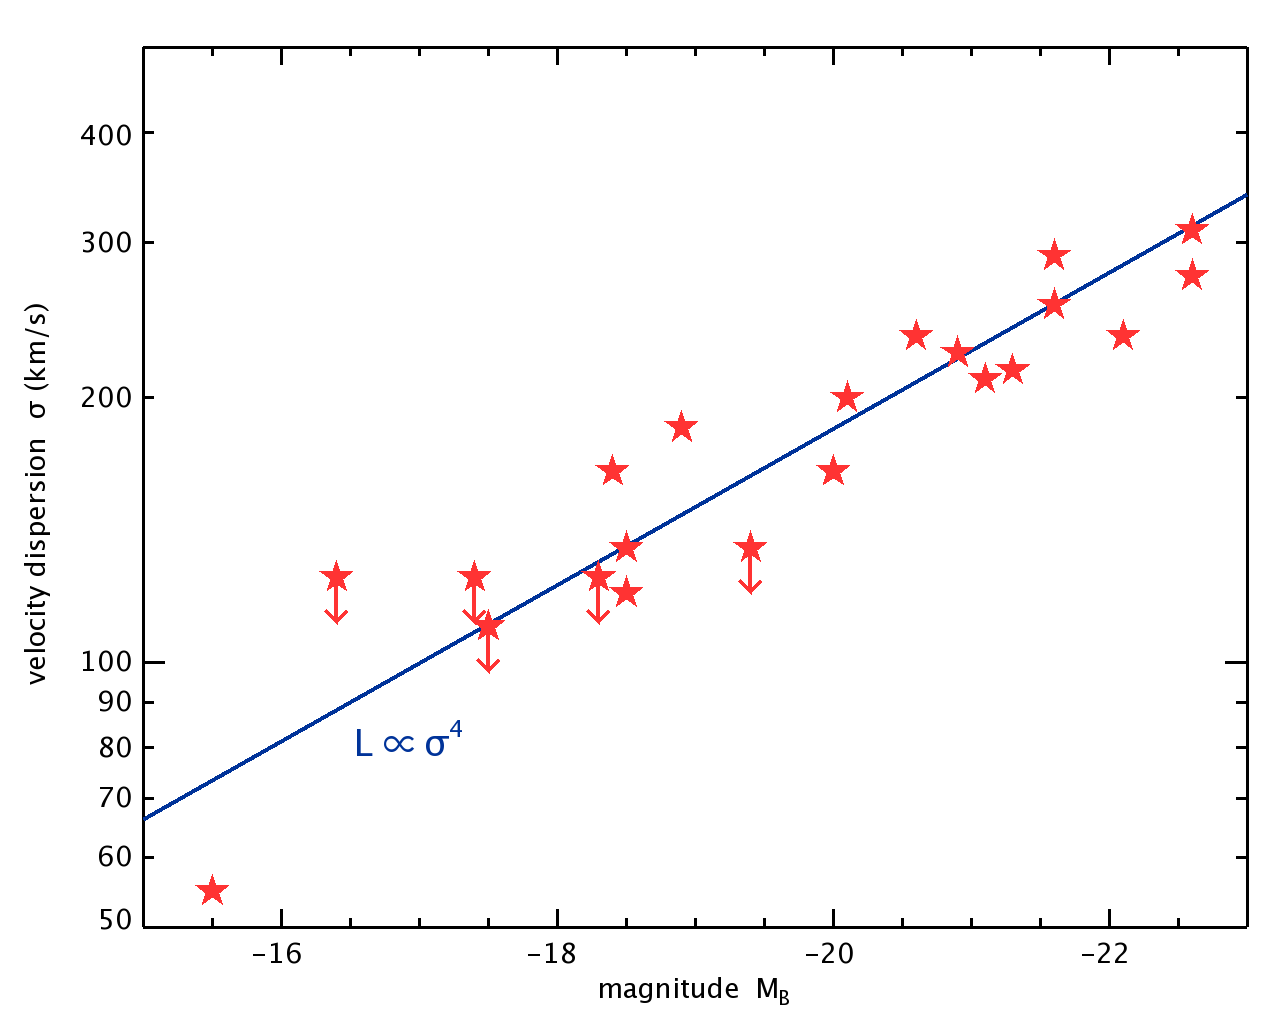
\includegraphics[width=1.0\linewidth]{Faber_Jackson.png}
	\caption{Faber-Jackson 关系,图源 Wikipedia}  \label{fig:Faber-Jackson}
\end{figure}

与 Tully-Fisher 关系不同, Faber-Jackson 关系可以从图上看到明显的展宽,因为
实际上的光度
\begin{equation}
    L = \left\langle I \right\rangle \times \pi \left\langle R \right\rangle ^2 \propto \sigma^\alpha
\end{equation}
其中 $\left\langle I \right\rangle$ 是椭圆星系的面亮度, $\alpha$ 是待定参数。
% 中单位面积上恒星的平均光度
更加完善的是 光度、速度弥散、半径三个参数之间的
“基本面” (Fundamental Plane) 关系。

半径与速度弥散、面亮度有关,记幂指数分别为 $a$, $b$. 
\begin{equation}
    R\propto \sigma_0^a \left\langle I \right\rangle ^b
\end{equation} 
则有
\begin{equation}
    \log R_{e}=a \log \sigma_{0}+b \log \langle I\rangle_{e}+\text { constant }
\end{equation}
其中加上了下标$e$表示有效半径和有效面亮度。

我们可以从维里定理来简单推导这个关系。

维里定理
$K = -\frac{1}{2}U$,
代入动能和势能得到
\begin{eqnarray}
        \left\langle v^2 \right\rangle &=& \frac{GM}{\left\langle R \right\rangle } = \frac{G(M/L)}{\left\langle R \right\rangle} \times L \\ 
        &=& \frac{G(M/L)}{\left\langle R \right\rangle} \times \left\langle I \right\rangle \times \pi \left\langle R \right\rangle ^2 = \pi G (M/L) \left\langle I \right\rangle \left\langle R \right\rangle
\end{eqnarray}
所以
\begin{equation} \label{eq:RvI}
    \left\langle R \right\rangle = \frac{1}{\pi G} \left\langle v^2 \right\rangle (M/L)^{-1} \left\langle I \right\rangle ^{-1}
\end{equation}

有效半径 $R_e$ 的定义是 包含一半亮度的半径 (effective radius enclosing half of the light),  
$\sigma_0$ 是视线方向经过质量加权的速度弥散, (mass-weighted) velocity dispersion along the line of sight.

记
$\left\langle R \right\rangle = \kappa_R R_e $,
$\sigma_0 = \kappa_v \sqrt{\left\langle v^2 \right\rangle } $,
代入 \refeq{eq:RvI} 得
\begin{equation}
    R_e = \frac{1 }{\pi G \kappa_R \kappa_v^2} \sigma_0^2 \left\langle I \right\rangle ^{-1} (M/L)^{-1} \propto \sigma_0^2 \left\langle I \right\rangle ^{-1} 
\end{equation}

解释了基本面关系,
给出 $a=2$, $b=-1$ 的结果,
实际观测中 $a\sim 1.2-1.5$, 与波段有关,$b\sim -0.8$.

维里定理给出的结果是接近的,差异在于我们的推导做了很多假设,比如假设 $\kappa_R$, $\kappa_v$ 是常数,假设 $(M/L)$ 与 $\sigma_0$ 和 $\left\langle I \right\rangle$ 无关。一个
修正是假设 $(M/L) \propto \sigma_0^\alpha \left\langle I \right\rangle ^\beta$.

\subsection{椭圆星系形成机制}

椭圆星系形成机制还在研究中,以下因素可能会影响形成盘星系还是椭圆星系:
\begin{itemize}
    \item 角动量大小。角动量大的容易形成盘星系,小的容易形成椭圆星系。
    \item 密度。密度大的塌缩较快,更容易形成椭圆星系。密度小的塌缩较慢,有足够多的时间在角动量作用下压缩成盘星系。
\end{itemize}

形成过程:
\begin{itemize}
    \item 巨塌缩 (Monolithic Collapse) : 巨大质量的气体团 在塌缩、冷却、恒星形成、反馈等过程下直接形成椭圆星系或盘星系。
    \item 多层次星系并合 (Hierarchical Merging Scenario) :小质量星系经过多次碰撞并合形成大的星系。
\end{itemize}


\end{document}
